\begin{titlepage}
\sffamily\color{BookInk}\setlength{\parindent}{0pt}
\vspace*{13mm}
{\small\color{BookAccent}\ifdefined\FrenchBook INFORMATION\quad IMAGES\quad APPRENTISSAGE\else INFORMATION\quad IMAGES\quad LEARNING\fi\par}
\vspace{16mm}
{\fontsize{36}{43}\selectfont\bfseries\parbox{.92\linewidth}{\raggedright\BookTitle}\par}
\vspace{10mm}{\color{BookAccent}\rule{32mm}{1.2pt}\par}
\vspace{12mm}{\Large\BookAuthor\par}
\vspace{4mm}{\normalsize\BookResearchUnit\par\BookInstitution\par}
\vspace{6mm}{\small\color{BookMuted}\BookEditionDate\par}
\vfill
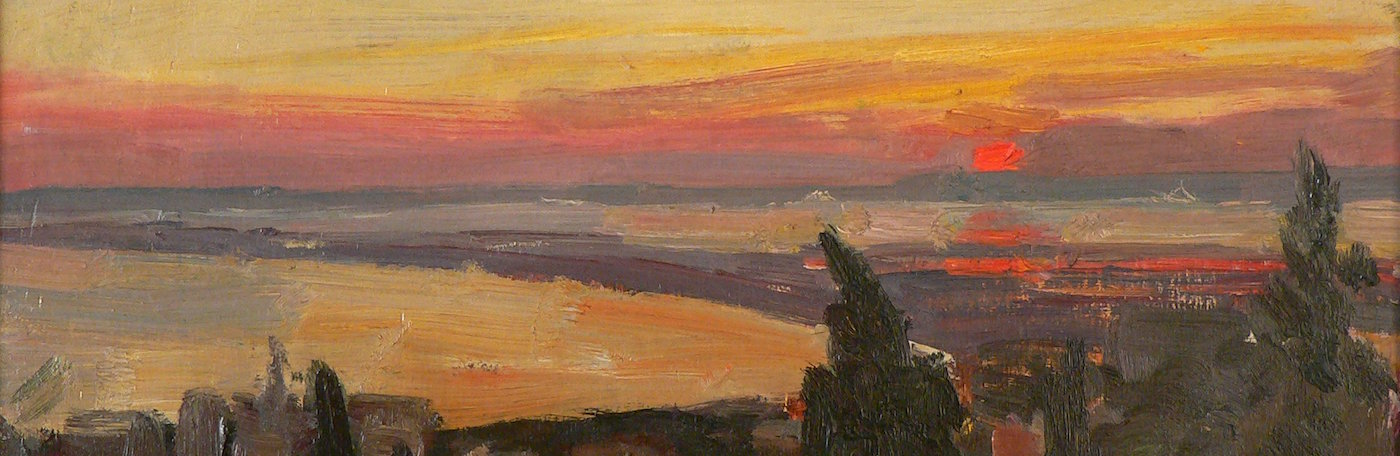
\includegraphics[width=\linewidth]{chapter-book-cover/sunset-landscape/artwork.jpg}
\vspace{2mm}{\scriptsize\color{BookMuted}\ifdefined\FrenchBook Couverture : détail d’un tableau de \else Cover: detail of a painting by \fi\href{https://www.louispeyre.com/}{Louis Peyré (1923--2012)}.\par}
\vfill
{\small\ifdefined\FrenchBook Une introduction aux idées mathématiques qui permettent de représenter, traiter et apprendre à partir des données.\else An introduction to the mathematical ideas behind representing, processing and learning from data.\fi\par}
\vspace{9mm}{\small\url{https://mathematical-tours.github.io/book-basics/}\par}
\end{titlepage}
